% Benchmark A: two unit blocks in compression (flat frictionless contact
% vs bonded shared-node reference)
\documentclass[border=8pt]{standalone}
\usepackage{tikz}
\usetikzlibrary{arrows.meta,patterns.meta}

\newcommand{\rollersym}[3]{%
  \begin{scope}[shift={(#1,#2)}, rotate=#3]
    \draw[fill=white] (0,0) -- (-0.09,0.16) -- (0.09,0.16) -- cycle;
    \draw[fill=white] (-0.075,0.20) circle (0.022);
    \draw[fill=white] (0.075,0.20) circle (0.022);
    \draw (-0.11,0.235) -- (0.11,0.235);
    \draw[gray] (-0.13,0.245) -- (-0.10,0.285);
    \draw[gray] (-0.06,0.245) -- (-0.03,0.285);
    \draw[gray] (0.01,0.245) -- (0.04,0.285);
    \draw[gray] (0.08,0.245) -- (0.11,0.285);
  \end{scope}
}

\begin{document}
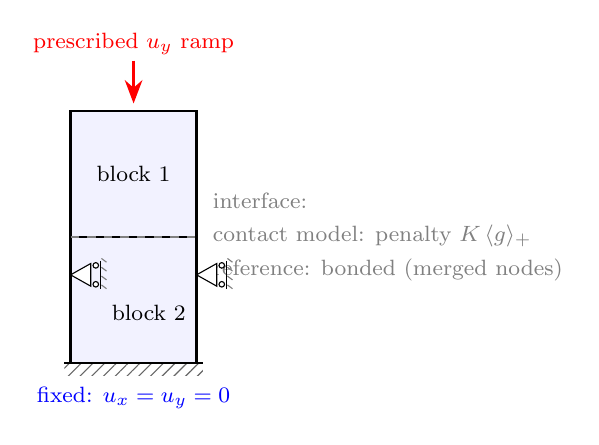
\begin{tikzpicture}[>={Stealth}, scale=1.6]

  % ---- two unit blocks ----
  \draw[thick, fill=blue!5] (0,0) rectangle (1,1);
  \draw[thick, fill=blue!5] (0,1) rectangle (1,2);
  \node at (0.62, 0.4) {\footnotesize block 2};
  \node at (0.5, 1.5) {\footnotesize block 1};

  % ---- prescribed u_y on top (downward arrow) ----
  \draw[red, very thick, ->] (0.5, 2.4) -- (0.5, 2.06);
  \node[above, red, inner sep=2pt] at (0.5, 2.4)
    {\footnotesize prescribed $u_y$ ramp};

  % ---- fixed ground below ----
  \fill[pattern={Lines[angle=45, distance=3pt]}, pattern color=black!60]
    (-0.05, -0.1) rectangle (1.05, 0.0);
  \draw[thick] (-0.05, 0.0) -- (1.05, 0.0);
  \node[below, blue, inner sep=3pt] at (0.5, -0.12)
    {\footnotesize fixed: $u_x = u_y = 0$};

  % ---- contact interface ----
  \draw[dashed, gray] (0, 1) -- (1, 1);
  \node[right, gray, inner sep=3pt, align=left] at (1.06, 1.0)
    {\footnotesize interface:\\
     \footnotesize contact model: penalty $K\,\langle g\rangle_+$\\
     \footnotesize reference: bonded (merged nodes)};

  % ---- side rollers: u_x = 0 on the outer edges ----
  \rollersym{0}{0.7}{-90}
  \rollersym{1}{0.7}{-90}

\end{tikzpicture}
\end{document}
